%!TEX root = minta_dolgozat.tex
%%%%%%%%%%%%%%%%%%%%%%%%%%%%%%%%%%%%%%%%%%%%%%%%%%%%%%%%%%%%%%%%%%%%%%%
\chapter{Darabolás}\label{ch:SEGMENT}
%%%%%%%%%%%%%%%%%%%%%%%%%%%%%%%%%%%%%%%%%%%%%%%%%%%%%%%%%%%%%%%%%%%%%%%

Annak érdekében, hogy megtaláljunk egy forgalmi táblát egy képen, szegmentációt alkalmaztam. A szegmentáció az a folyamat, amikor kisebb képeket vágunk ki egy nagyobb képből. \cite{7}

Több különböző módszer létezik a szegmentálás végrehajtására. Az általam alkalmazott véletlenszerű kiválasztáson alapszik. Véletlenszerű téglalapokat generálok és vágom ezeket ki az eredeti képből.

Mivel a valós környezetből vett képek több forgalmi táblát is tartalmazhatnak, fontos hogy az egész képet bejárják ezek a darabok. Az által hogy nagy számban generálok ilyen darabokat, biztosítom, hogy nagy valószínűséggel megtaláljam a képen levő forgalmi táblákat. A táblák mérete is változik attól függően, hogy milyen távolságra van a fényképezőtől, ezért arra is figyelnem kellett, hogy a kivágott darabok mérete széles tartományban mozogjon.

Az által, hogy véletlenszerűen választom ki a vizsgálandó részeket az eredeti képből, ezeknek nagy része olyan kép lesz, ami nem tartalmaz forgalmi táblát vagy csak részlegesen fogja azt tartalmazni. Ez az oka annak, hogy a neurális háló akkor is megfelelően kell osztályozza a táblát ha csak 70-80\% látszik belőle.

\begin{figure}[h]
\centering

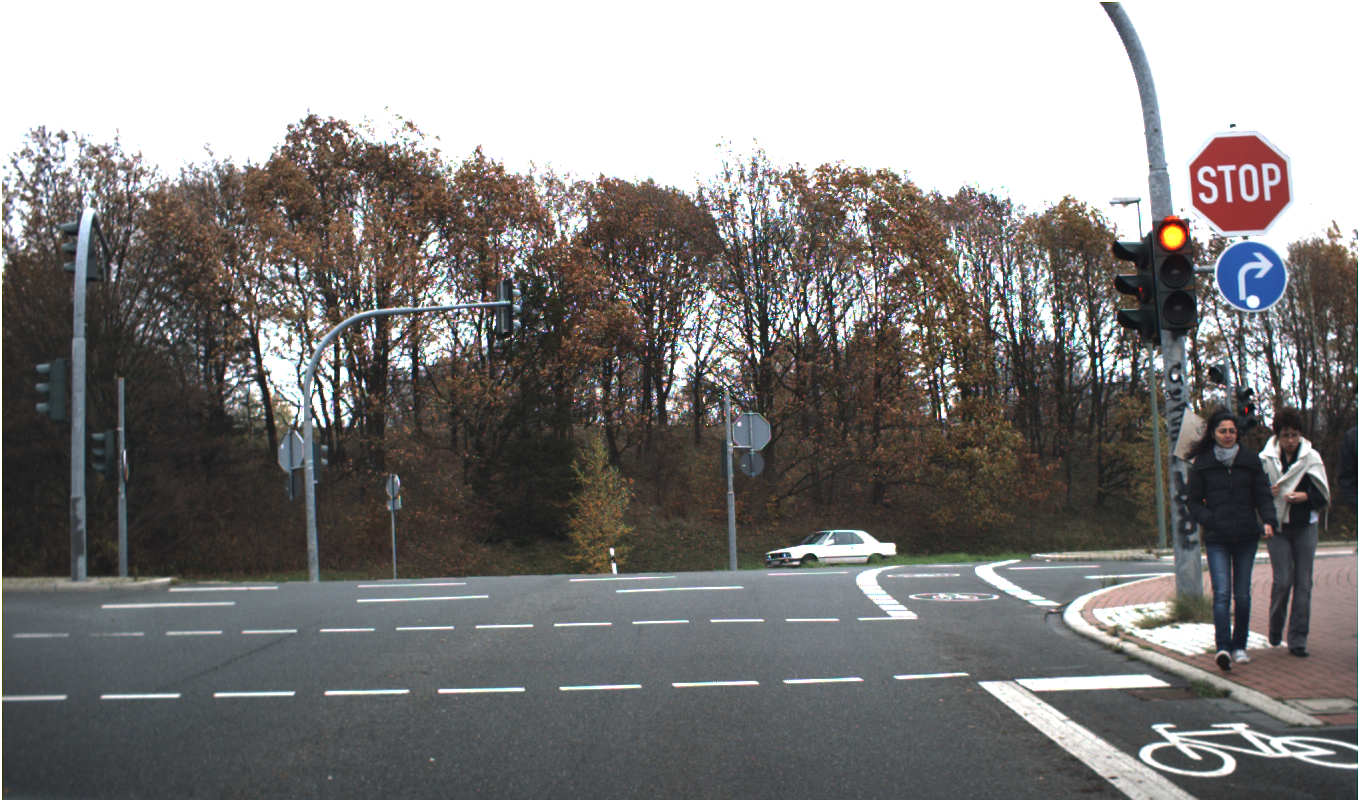
\includegraphics[scale=0.4]{images/testImage2}
\caption{Szegmentálás előtti kép}

\label{fig:testImage2}
\end{figure}

\makeatletter
    \setlength\@fptop{0\p@}
\makeatother

\begin{figure}[htbp]
\centering

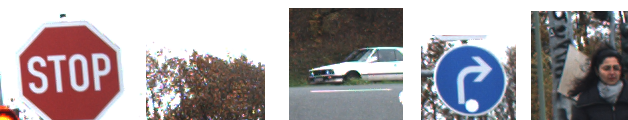
\includegraphics[scale=1]{images/segments}
\caption{Példa szegmentálás utáni képekre}

\label{fig:segments}
\end{figure}